% Describe how the experiments are performed

\subsection{Tyrimo metodika}\label{sec:exp:methodology}

Visa tyrimo metodika pavaizduota \ref{fig:methodology} pav. Tyrimui pasirinktas \SLEIPNIR \cite{al-dujailiAdversarialDeepLearning2018} duomenų rinkinys, kuriame yra $34995$ kenkėjiškų programų ir $19696$ nekenkėjiškų programų pavyzdžių, užkoduotų $22761$-mačiais dvejetainiais vektoriais. Iš šio rinkinio pasirinkta po $1500$ unikalių kenkėjiškų ir nekenkėjiškų programų pavyzdžių paliekant pirmas $200$ komponenčių -- taip gaunamas subalansuotas duomenų rinkinys. Šis rinkinys toliau skeliamas į mokymo ir testavimo aibes santykiu $4:1$.
Eksperimentams atlikti paruošiamos šios priemonės:
\begin{enumerate}
    \item Testavimo duomenų aibė, iš kurios sudaromas trijų tipų programų požymių srautas: nekenkėjiškos, kenkėjiškos, kenkėjiškos-obfuskuotos.
    \item \textit{MalGAN} \cite{huGeneratingAdversarialMalware2017} \gls{ae} generatorius. Pasirinkimo motyvacija pateikiama \ref{sec:method:malgan} poskyryje.
    \item Kenkėjiškų programų detektorius (klasifikatorius). Naudojamas \gls{gbdt} modelis.
    \item \Glsplko{adversarial} aptikimo komponentas
    \begin{itemize}
        \item Naudojantis originalius požymius.
        \item Naudojantis \gls{mca} transformuotus požymius \skyrius{sec:method}.
    \end{itemize}
\end{enumerate}

\noindent
Su šiais įrankiais atliekami 4 eksperimentai \textbf{aplinkoje su \glsplkuo{adversarial}}:
    \begin{enumerate}
        \item Bazinis atvejis -- originalaus klasifikatoriaus tikslumo nustatymas.
        \item Klasifikatoriaus, naudojančio \gls{mca} transformuotus požymius, tikslumo nustatymas.
        \item Klasifikatoriaus praplėtimo su modifikuoto \LIME metodo pritaikymu \glsplko{adversarial} aptikimui tikslumo nustatymas.
        \item Klasifikatoriaus praplėtimo su \LIME ir \gls{mca} metodų sinteze \glsplko{adversarial} aptikimui tikslumo nustatymas.
    \end{enumerate}

Visų tyrime atliekamų klasifikacijų kokybė matuojama taikant preciziškumo \angl{precision}, atkūrimo \angl{recall} ir F1 metrikas bei vertinamas bendras tikslumas \angl{accuracy}. 

\begin{figure}[h]
    \centering
    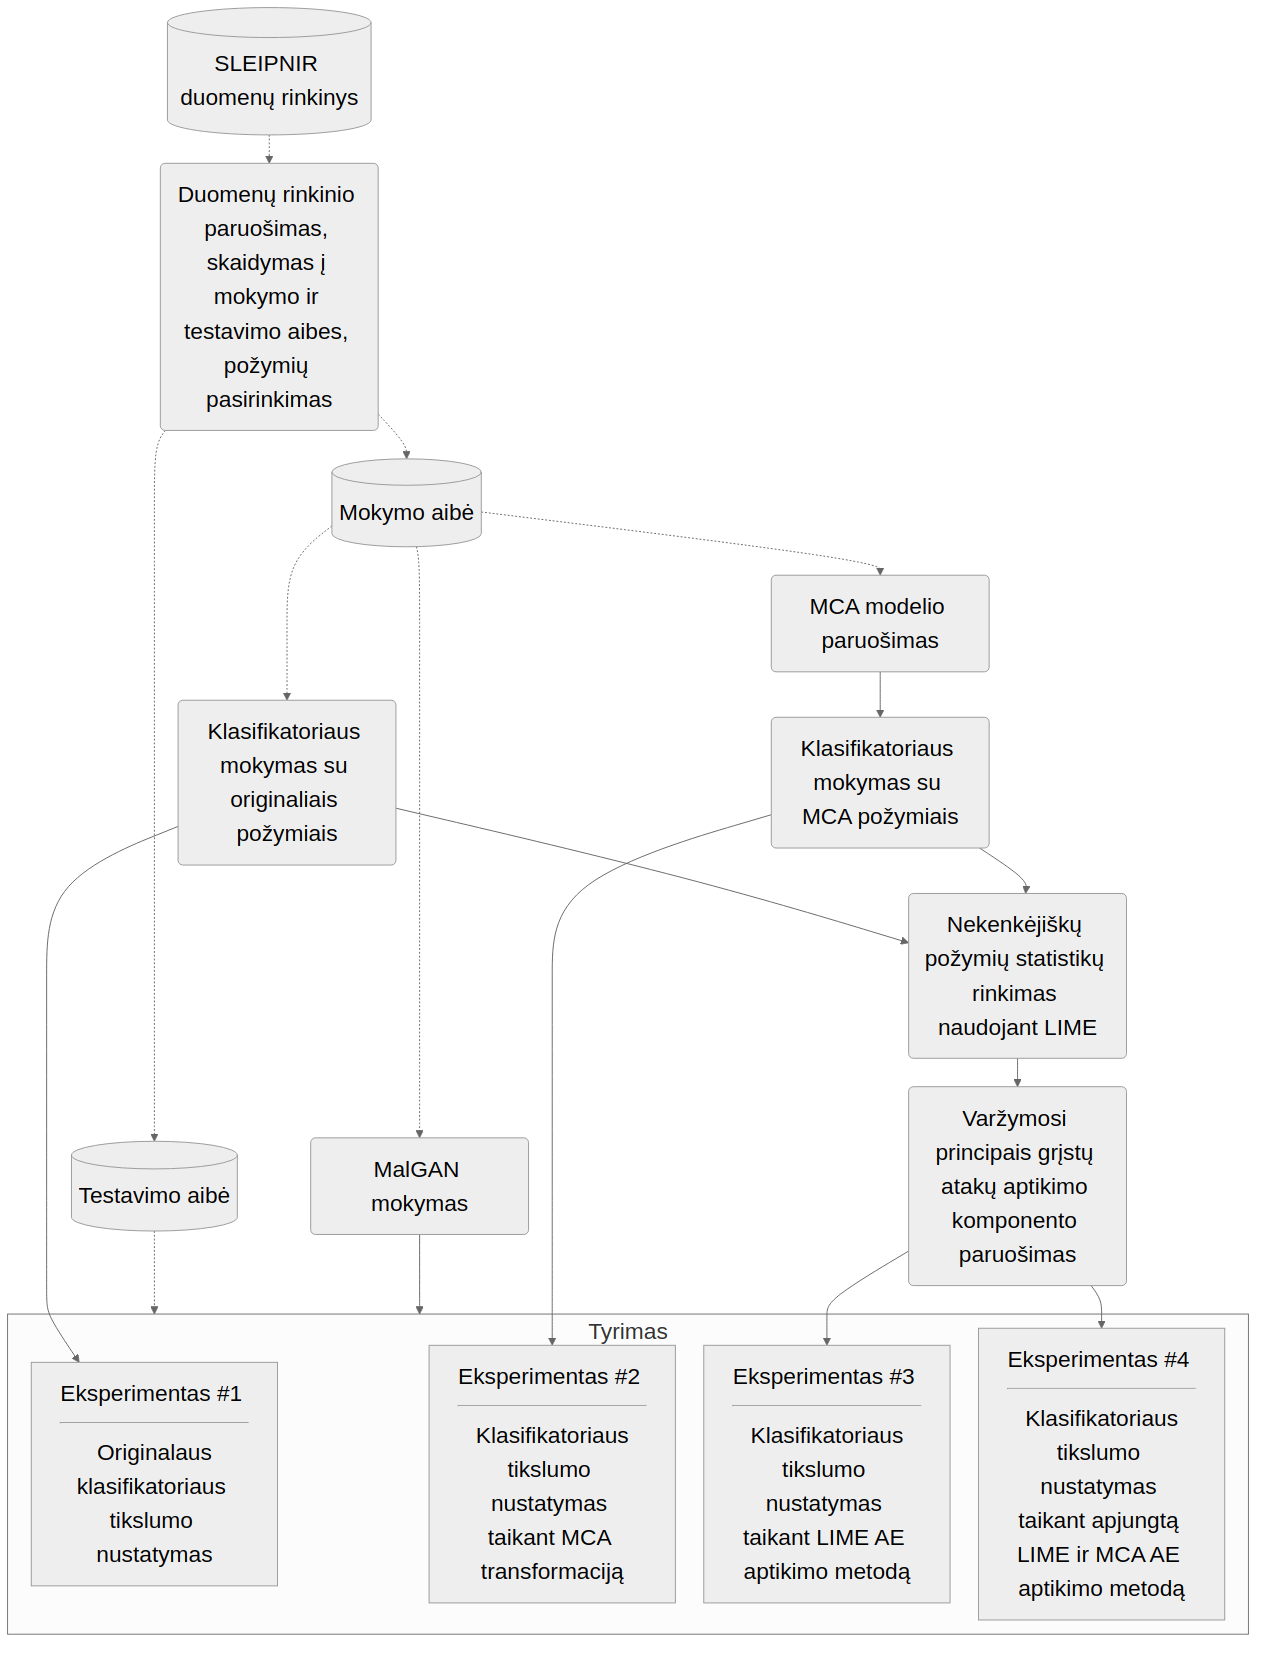
\includegraphics[width=0.76\textwidth]{images/methodology.png}
    \caption{Tyrimo metodika}
    \label{fig:methodology}
\end{figure}

\subsection{\Glsplko*{adversarial} \glsko*{framework} pasirinkimas}\label{sec:method:malgan}

Tyrimui pasirinktas \refFramework{MalGAN} \gls{framework} dėl šių priežasčių:
\begin{itemize}
    \item \gls{gan} yra vieni iš perspektyviausių ir efektyviausių \gls{ml} modelių \gls{ae} generavimui.
    \item \textit{MalGAN} yra plačiai naudojamas kaip bazinis modelis tolimesniems tyrimas, yra kelios atviro kodo repozitorijos\footnote{Šiam tyrimui pasirinkta https://github.com/ZaydH/MalwareGAN repozitorija, kaip pradinis \textit{MalGAN} įgyvendinimas}, įgyvendinančios šį \glska{framework}.
    \item \textit{MalGAN} naudoja dvejetainius požymių vektorius. Būtent tokie požymiai turėtų kelti sunkumų esamiems \gls{ae} aptikimo metodams \poskyris{sec:method:mods}.
\end{itemize}

\clearpage
\subsection{\gls*{mca} komponenčių pasirinkimas}\label{sec:method:mca_comp_selection}
Komponenčių pasirinkimas yra \ref{fig:methodology} pav. minimo \gls{mca} modelio paruošimo dalis. Komponenčių pasirinkimui, \ty~jų kiekio pasirinkimui, nėra apibrėžto \enquote{teisingo} metodo \cite{abdiPrincipalComponentAnalysis2010}. Dažniausiai siūlomi metodai yra tik didesnių už $1$ tikrinių reikšmių pasirinkimas ir \textit{alkūnės} \angl{scree / elbow} metodas. Šie metodai netiko, nes juos taikant paliktos \gls{mca} komponentės nepaaiškintų net pusės visos \glsko{inertia}: visos tikrinės reikšmės analizuojamuose mokymo duomenyse yra $<1$, o alkūnės taške sukaupta \gls{inertia} yra $\num{47,62}\;\%$ \zr{fig:inertia}. Taigi, pasirinkti 2 nestandartiniai \gls{mca} komponenčių kiekio kriterijai: 

\noindent
\begin{minipage}[l]{0.48\textwidth}
    \vspace{-2cm}
    \begin{itemize}[leftmargin=*]
        \item sukaupta \gls{inertia} $\ge 75\;\%$,
        \item išmokyto klasifikatoriaus tikslumas $\hat{a}$ nemažesnis nei originalaus klasifikatoriaus tikslumas $a$ $5\;\%$ intervale ($\hat{a} \ge a - 5\;\%$), kai įvesčių srautas normalus (nėra obfuskuotų programų požymių -- \gls{ae}). Šiuo atveju $\hat{a} \ge \num{\mathOp{\accNoAttackNormal - 0.05}}$ \Zr{tbl:safe:original:metrics}
    \end{itemize}
\end{minipage}
\hspace{0.02\textwidth}
\begin{minipage}{0.5\textwidth}
    \centering
    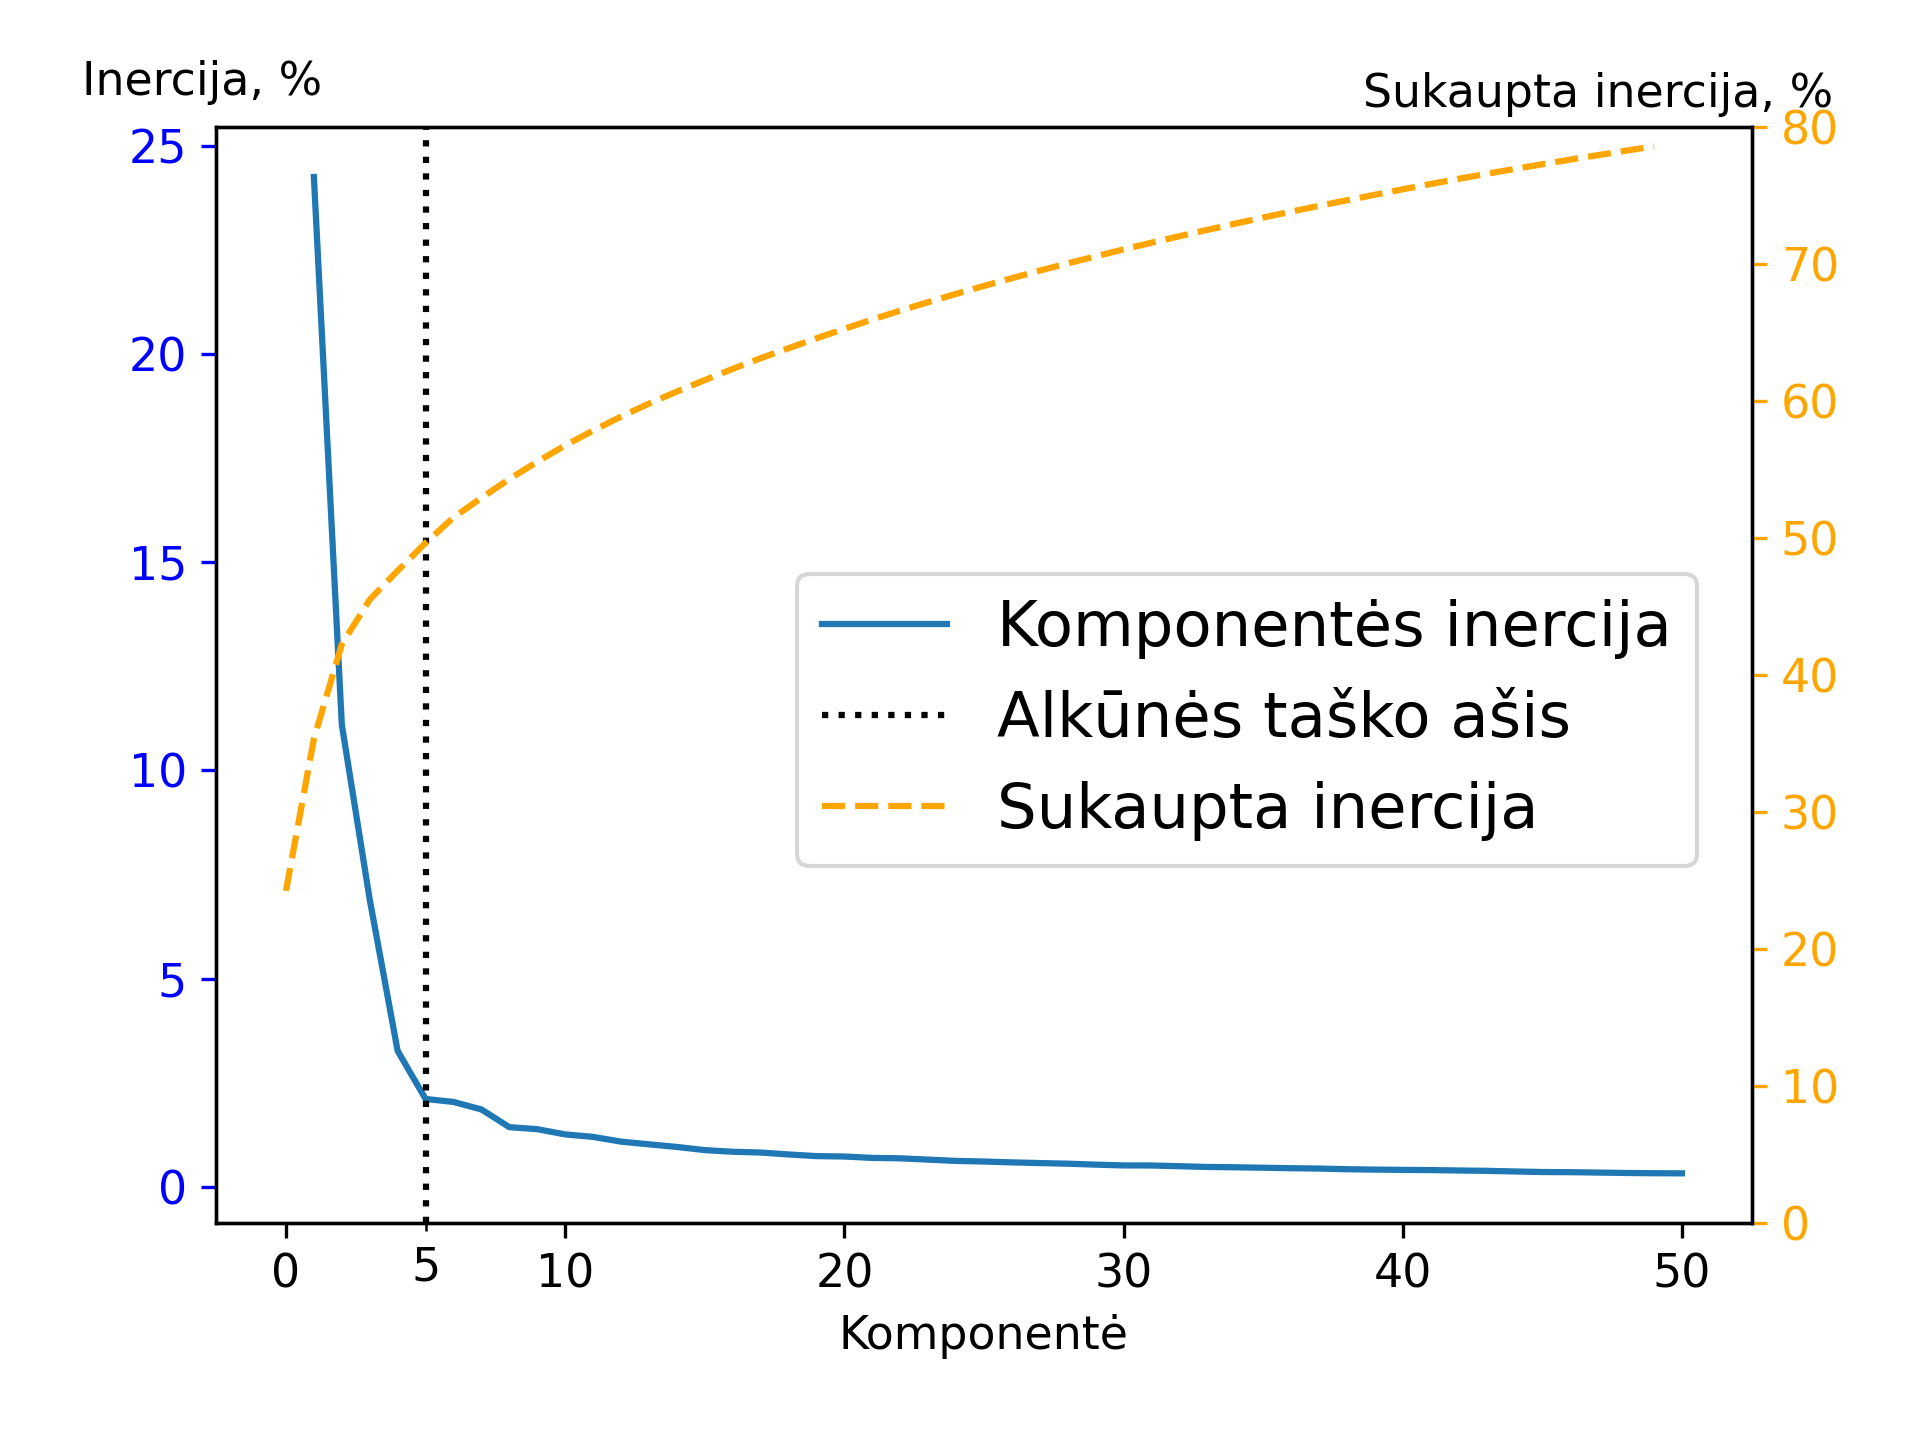
\includegraphics[width=\textwidth]{images/scree.png}
    \vspace{-1cm}
    \captionof{figure}{\textit{Alkūnės} analizė \gls{mca} inercijai}
    \label{fig:inertia}
\end{minipage}

\begin{table}[h]
    \centering
    \caption{Originalaus\textsuperscript{\ref{footnote:original_classifier}} klasifikatoriaus metrikos, kai nevykdoma \gls{adversarial}}
    \exptable[\accNoAttackNormal]{tables/original_no_attack.csv}
    \label{tbl:safe:original:metrics}
\end{table}
\begin{table}[h]
    \centering
    \caption{\gls{mca} klasifikatoriaus metrikos, kai nevykdoma \gls{adversarial}}
    \exptable[\accNoAttackMca]{tables/mca_no_attack.csv}
    \label{tbl:safe:mca:metrics}
\end{table}

\def\accumulatedInertia{$78,57\;\%$}

\ref{tbl:safe:mca:metrics}-oje lentelėje pavaizduotos \gls{mca} transformacijos klasifikatoriaus metrikos gaunamos pasirinkus 50 komponenčių (suspaudimo santykis $4:1$), kurių sukaupta \gls{inertia} yra \accumulatedInertia. Kadangi \accumulatedInertia $\;> 75\;\%$ ir $\num{\accNoAttackMca} > \num{\mathOp{\accNoAttackNormal - 0.05}}$, abu \gls{mca} komponenčių kiekio kriterijai yra tenkinami.

% --- PCA/MCA
% Show graphs of 2 best components (~30% of inertia)
% Show knee analysis of 50 then 9 components